\graphicspath{{chapters/11/images}}
\chapter{Stochastic methods for parameter estimation}

\section{Introduction}
Stochastic methods are often used when we cannot compute the gradient.
With the same parameters, stochastic methods can produce dramatically different results, as it can be seen in figure \ref{fig:res}.

\begin{figure}[H]
  \centering
  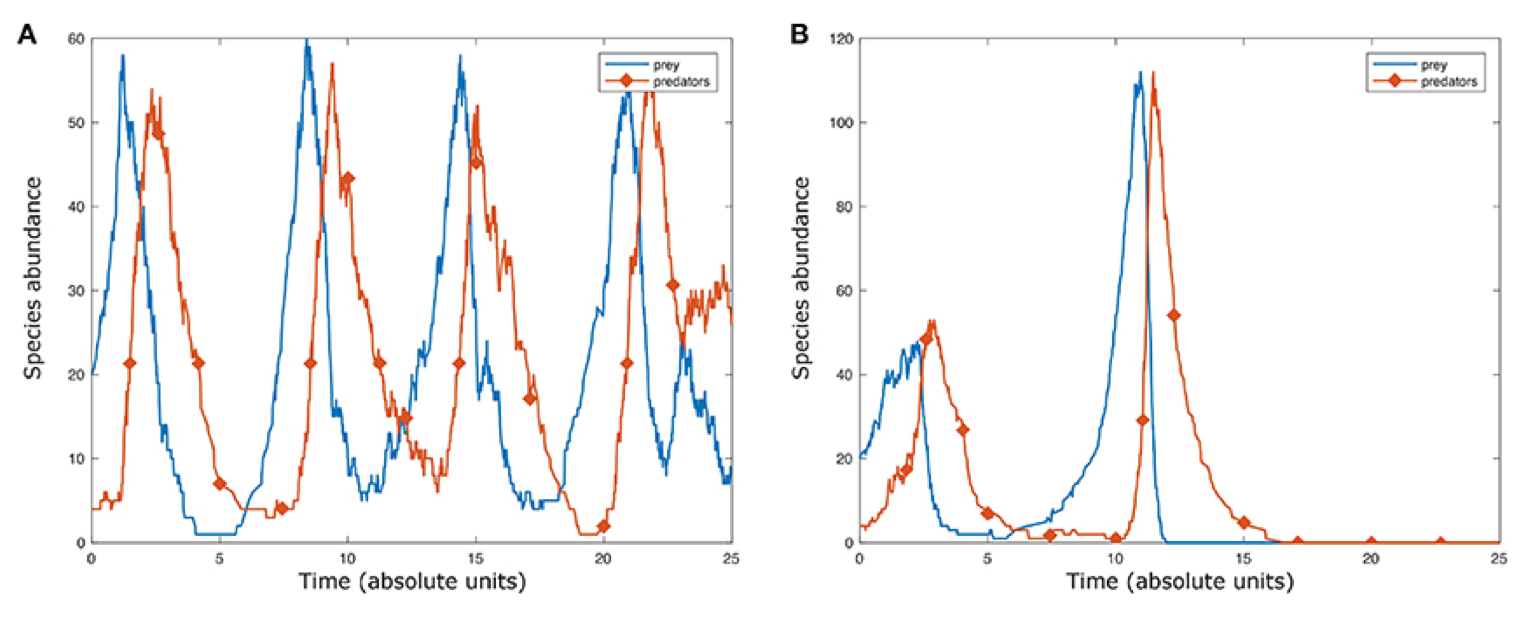
\includegraphics[width=\textwidth]{stoch_LV.png}
  \caption{Lotka-Volterra stochastic simulation results. In B we witness
  preys and predators extinction, it is the output of a simulation
  performed with the same model and parameters as A.}
\label{fig:res}
\end{figure}

Instead of following the gradient informations are collected in a manner resembling natural selection.
Monte Carlo Methods are dated around 1949, the name comes from casinos.
In order to use MCM to do inference, Metropoli and Hastings developed a specific algorithm in 1970.

\section{Markov Chain Monte Carlo (MCMC)}
MCMC is a chain of events where the current state depends on the previous one and on the transition probability.
Running MCMC long enough they will reach a stable point.
$x^{(i)}$ is a random variable or stochastic process that takes only discrete values $\{x_1,\dots,x_s\}$.
Let $p(x)$ be the probability distribution of $x$.

  \subsection{Markov chain}
  $x^{(i)}$ is a Markov Chain if:

  $$p(x^{(i)}|x^{(i-1)},\dots,x^{(1)})=T(x^{(i)}|x^{(i-1)})$$

    \subsubsection{Homogeneity}
    A Markov chain is homogenous if $T(x^{(i)})x^{(i-1)}=T$,
    So that the transition matrix is constant.

  \subsection{Example}
  Let $3$ states as in figure \ref{fig:MCMCexmple}.

  \begin{figure}
    \centering
    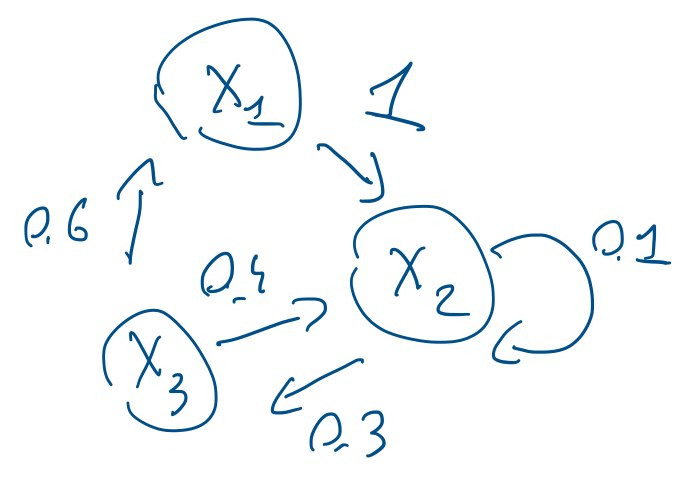
\includegraphics[width=0.3\textwidth]{mcmc.png}
    \caption{MCMC example}
    \label{fig:MCMCexample}
  \end{figure}

  The homogeneous transition matrix:

  $$T = \begin{bmatrix}0 & 1 & 0\\0 & 0.1 & 0.9\\ 0.6 & 0.4 & 0\\\end{bmatrix}$$

  And the states:

  $$\pi_1=\begin{pmatrix}0.5 & 0.2& 0.3 \end{pmatrix}$$

  The next probability of being in the three states is given by

  $$\pi_1 \cdot T=\begin{pmatrix}0.3\cdot0.6, & 0.5+0.02+0.12,& 0.18 \end{pmatrix} = \begin{pmatrix}0.18, & 0.64,& 0.18 \end{pmatrix}$$

  Iterating enough time a fixed distribution will be reached.

  \subsection{Invariant distribution}
  The invariant distribution if a fixed distribution reached after enough Monte Carlo iterations.
  The objective is to build a Markov chain whose invariant distribution is the distribution of the unknown parameters.
  For example, in the previous example, the invariant distribution will be:

  $$p(x)=\dots = \begin{pmatrix} 0.2213 \\ 0.4098 \\ 0.3689\end{pmatrix}^T$$

  \subsection{Irreducible matrices}
  A stochastic matrix is irreducible if its graph does not contain unconnected sub-graphs.
  If $T$ is an irreducible transition matrix and is aperiodic the Markov chain has an invariant distribution.
  The probability distribution has to be linked with the model.

  \subsection{Monte Carlo sampling}
  Monte Carlo refers to a family of methods developed for sampling.
  In particular, the output of a Monte Carlo method are independent and identically distributed random variables $\{x^{(i)}\}_{i>0}$ from a known density $p(X)$.
  The samples can be used to ``estimate or approximate'' a target density or distribution.
  Known distributions are exploited to approximate the unknown distribution of interest.
  Given enough samples, $p$ can be approximated as:

  $$p_N(x)= \frac{1}{N}\sum^N_{i=1}\delta_{x^{(i)}}(x)$$

  With:

  $$\delta_{x^{(i)}}(x)= \begin{cases}1, & x=x^{(i)} \\ 0, & \text{elsewhere}\end{cases}$$

  This is often used to approximate ``hard'' integrals.
  An integral with a finite sum of values, can be obtained as:

  $$I_N(f)=\frac{1}{N} \sum^N_{i=1} f(x^{(i)})$$

  The function is being evaluated as some points and the mean is an integration of the integral.
  This equation converges to the real integral by the law of large numbers:

  $$I_N(f)=\frac{1}{N} \sum^N_{i=1} f(x^{(i)})  \xrightarrow[N \rightarrow \infty  ]{}   I(f)= \int_x f(x)p(x)dx$$

  This is better than the output of the least square problem as it gives information about the shape of the distribution.

\section{Sampling a distribution}
Let $p$ be a known probability distribution up to a proportionality constant.
It is usually preferred to sample from a well-known distribution, like for example the one in \ref{fig:bimodal}.

$$q(x)\text{ such that }\exists M>0$$

$$p(x) \leq M q(x)$$


\begin{figure}
  \centering
  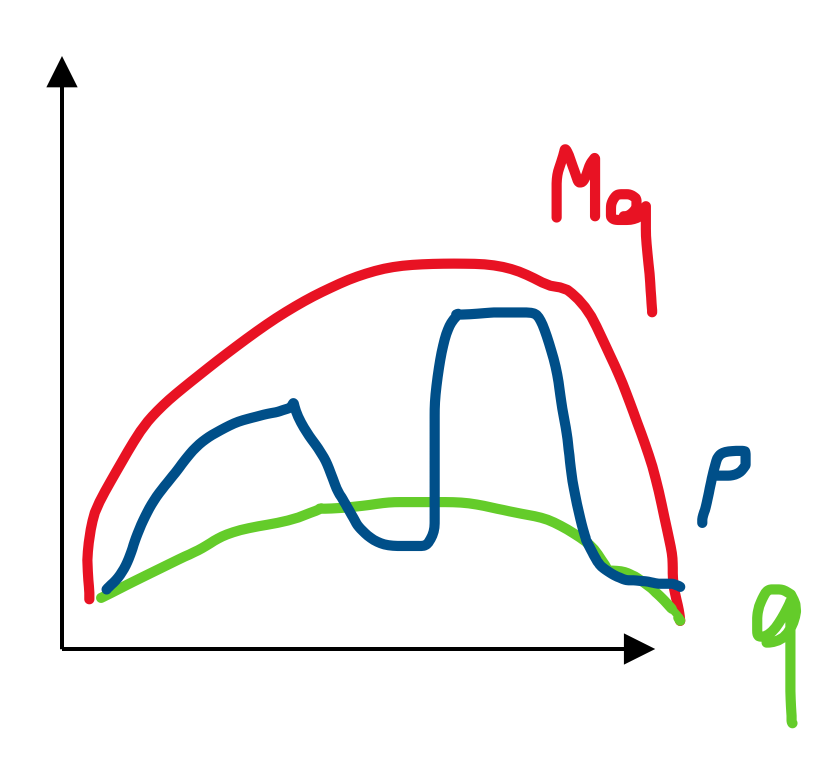
\includegraphics[width=0.3\textwidth]{distribution.png}
  \caption{Example: bimodal distribution}
  \label{fig:bimodal}
\end{figure}

Values from $q$ are extracted if they are smaller than $Mq$.
Each time information about $p$ are collected from $q$.

  \subsection{Rejection sampling algorithm}
  A rejection sampling implementation is outlined in algorithm \ref{algo:rejection-sampling}.

  \begin{algorithm}[H]
\DontPrintSemicolon
\SetKwComment{comment}{$\%$}{}
\SetKw{Int}{int}
\SetKw{To}{to}
\SetKw{Return}{return}
\SetKw{Not}{not}
\SetKw{Input}{Input}
\SetKw{Output}{Output}
\SetKw{False}{false}
\SetKw{True}{true}
\SetKwData{Item}{item}
\SetKwFunction{Min}{min}
\SetKwFunction{Partitioning}{partitioning}
\SetKwFunction{TitleFunction}{Rejection sampling}

\caption{\protect\TitleFunction{}}
\label{algo:rejection-sampling}

\Input: $M$, $p(x)$ and $q(x)$\;

\Output: a random variable distributed according to $p$\;

$i = 1$\;
\Repeat{}{
	sample $x^{(i)}\sim q$, $u\sim norm(0,1)$\;
	\If{$u>\frac{p(x^{(i)})}{Mq(X^i)}$}{
		$i = i + 1$\;
	}
}

\end{algorithm}


  If the point is in the area between $p$ and $Mq$ is accepted.
  The further the ratio is from $1$, the smaller the chance of keeping the point.
  A known distribution $p$ is being used, then gradually what is known about it is removed in the following iterations.

\section{Metropolis Hastings}

Let $X$ be our current point, $q$ the proposal distribution and $p$ the
target distribution. $p$ can be an unnormalized density
($\int p > 1 \text{ but} \int p < \infty)$. Ideally we want to know $p$,
but if it is unknown we can still proceed. Let us call this function $h$
(non negative and positive integral).
\\
\\
\noindent
$X^*$ is the new candidate point. The trick of MH algorithm is to avoid
relying on probability, we use a function. We require info on $p$, but
not a probability.

\textbf{Metropolis ratio} $r_M(x,x^*)=\frac{h(x^*)}{h(x)}$

\textbf{Hastings ratio}
$r_H(x,x^*)=\frac{h(x^*)\cdot q(x^*|x)}{h(x)\cdot q(x|x^*)}$
\noindent
From the distribution, we want to measure how likely the previous value
is based on the current value. We are weighting our choices to
likeliness.


\subsubsection{MH algorithm}

Guess $x^{(i)}$

FOR $i=0$ to $N-1$

Sample $x^*$ from $q(\cdot|x^{(i)})$ and $u \in \mathcal{U}(0,1)$

IF $u < \min \{1, r_H(x,x^*) \}$

$x^{(i+1)}=x^{(*)}$

ELSE

$x^{(i+1)}=x^{(i)}$

END

END
\\
\\
\noindent
We sample from a proposal distribution and accept according to another
function i.e.~if it is more likely. If it is not more likely, we accept
it with a certain chance.
\\
\\
\noindent
MATLAB plot:

\begin{itemize}
\tightlist
\item
  right: histogram with the known distribution
\item
  left: MCMC oscillating between 0 and 10, recapitulates the
  distribution
\end{itemize}
\noindent
The procedure is really fast, takes less than a second. If instead of
extracting u and v from random distribution with an index, the result is
the same → ``thanks MATLAB, it is not necessary to prelocate anymore''
\\
\\
\noindent
If we employ a Gaussian distribution, the result is still good but not
as accurate as the previous one. We are adding complexity by introducing
the variance; by choosing a different value we can improve the result.
Pay attention to the fact that if we sample from a narrow distribution,
we risk focusing only on one of the two points.
\\
\\
\noindent
Everything we do has consequences!


\subsubsection{Visualization of MCMC}

\url{http://chi-feng.github.io/mcmc-demo/app.html?algorithm=RandomWalkMH\&target=banana}
\noindent
Green: accept, red: reject
\\
\\
\noindent
\underline{Target distribution = standard}

\begin{itemize}
\tightlist
\item
  GibbsSampling: collects points according to a certain direction from a
  starting point, it tries to rebuild a 2D Normal distribution.
\item
  AdaptiveMH: sample from a starting mean and accept or reject new
  points.
\item
  Random walk: more or less like MH. Even if the target distribution is
  not that difficult (bell shape), there are a lot of rejections
  initially.
\item
  DE-MCMC-Z: produces vectors.
\end{itemize}
\noindent
\underline{Target distribution = donut}

\begin{itemize}
\tightlist
\item
  SVGO: stochastic vector gradient descent, intermediate between
  gradient and stochastic.
\item
  EfficientNUTS (No-U-Turn samples): it creates many points, more
  complex but one of the best. In the end it will converge quite fast.
\item
  RandomWalk: needs more time to converge with respect to standard
  distribution.
\end{itemize}
\noindent
\underline{Target distribution = multimodal}

\begin{itemize}
\tightlist
\item
  RandomWalk: three initial points, it proposes a random perturbation.
\item
  AdaptiveMH: changes some of the parameters. Differently from the
  previous approach, the shape changes: instead of having a fixed search
  area, it evolves and adapts.
\end{itemize}


\subsubsection{How to link data and MH}

In LSQ, we used the function

$$
f(\theta)=\frac{1}{2}\sum^m_{j=1}r^2_j(\theta)=\frac{1}{2}\sum^m_{j=1}(y_j-m_j(t_i,\theta))^2
$$
\noindent
We can weight our residuals for their uncertainty:

$$
f_w(\theta)=\frac{1}{2}\sum^m_{j=1} \frac{r^2_j(\theta)}{\vartheta_j^2}
$$
\noindent
$\vartheta_j$= (for example) the standard deviation of that measured
point.
\\
\\
\noindent
We can use as function to link the parameters and the output, and be
non-negative: {[}where $Y$ is the vector of our observations{]}

$$
L(\theta|Y)=\exp(-f_w(\theta)) \geq 0
$$
\noindent
We can use this as $h$ in the MH algorithm.
\\
\\
\noindent
Metropolis ratio:

$$
r_H(\theta^*,\theta)=\frac{L(\theta^*)}{L(\theta)}=\frac{e^{-f_w(\theta^*)}}{e^{-f_w(\theta)}}=\exp(-f_w(\theta^*)+-f_w(\theta))
$$
\noindent
So since $f_w(\theta)\geq0$ we have that if
$f_w(\theta^*) > f_w(\theta) \Rightarrow r_H>1$ , we ACCEPT. Otherwise
we accept with a certain probability. This kind of function can be used
to link the new parameters with data.
\noindent
We can work with log-likelihood also here, we just look at
$f_w(\theta^*)$ and $f_w(\theta)$.


\subsection{Random walk MCMC}

Let us assume $\theta^*$ is sampled from
$\mathcal{N}(0,\mathcal{C})+\theta=\mathcal{N}(\theta,\mathcal{C})$
\\
\\
\noindent
We add a perturbation with $\mathcal{C}$, a known covariance matrix.
$\mathcal{C}$ can be fixed or adapted along the iterations.
\\
\\
\noindent
From the initial point we have a new candidate according to a
multivariate normal distribution; if the candidate is accepted, we we
will then restart evaluation from it. We are collecting some information
allowing us to shape the target distribution.


\subsubsection{Algorithm RW-MCMC ( C known)}

Initialize a matrix $D_\theta$ and a vector $V_L$

Randomly generate $\theta_1$

Compute $L(\theta_1)=L_1$

For $i=1:N$

	sample $Z \sim N(D,\mathcal{C})$

	compute $\theta_2=\theta_1+Z$

	compute $L_2=L(\theta_2)$

	compute $\text{ratio}=\frac{L_1}{L_2}$

	sample $u \sim\mathcal{U}(0,1)$

	IF $u < \text{ratio}$

		$L_1=L_2$

		$\theta_1=\theta_2$

	END

	IF $i > \text{warm-up}$

		$D_\theta=[D_\theta;\theta_1]$

		$V_L=[V_L;L_1]$

	END

END
\\
\\
\noindent
We want to find a good accept-reject tradeoff to reach a satisfactory
convergence.
\\
\\
\noindent
\textbf{Pros}

\begin{itemize}
\tightlist
\item
  the object function is evaluated once per iteration
\item
  the target distribution can be built form the samples
\item
  we only need the last point to restart
\item
  we can collect info on the model: variability on the output +
  sensitivity on parameters
\item
  random selection helps us to avoid local minima
\end{itemize}

\noindent
\textbf{Cons}

\begin{itemize}
\tightlist
\item
  convergence may be slow
\item
  sampling distribution may affect the results
\item
  each MCML cannot be parallelized
\item
  burn-time
\item
  diagnostics are heuristics
\end{itemize}


\subsubsection{Diagnostics}

We can exploit diagnostics to check if the parameters are good and
understand whether we are done or not.

\begin{enumerate}
\def\labelenumi{\arabic{enumi}.}
\tightlist
\item
  chain 1: expected MCMC plot
\item
  chain 2: we require a longer burn-in, we have not reached the target
  distribution
\item
  chain 3: we do not have enough information, the number of iterations
  is too small
\end{enumerate}

\begin{figure}
\centering
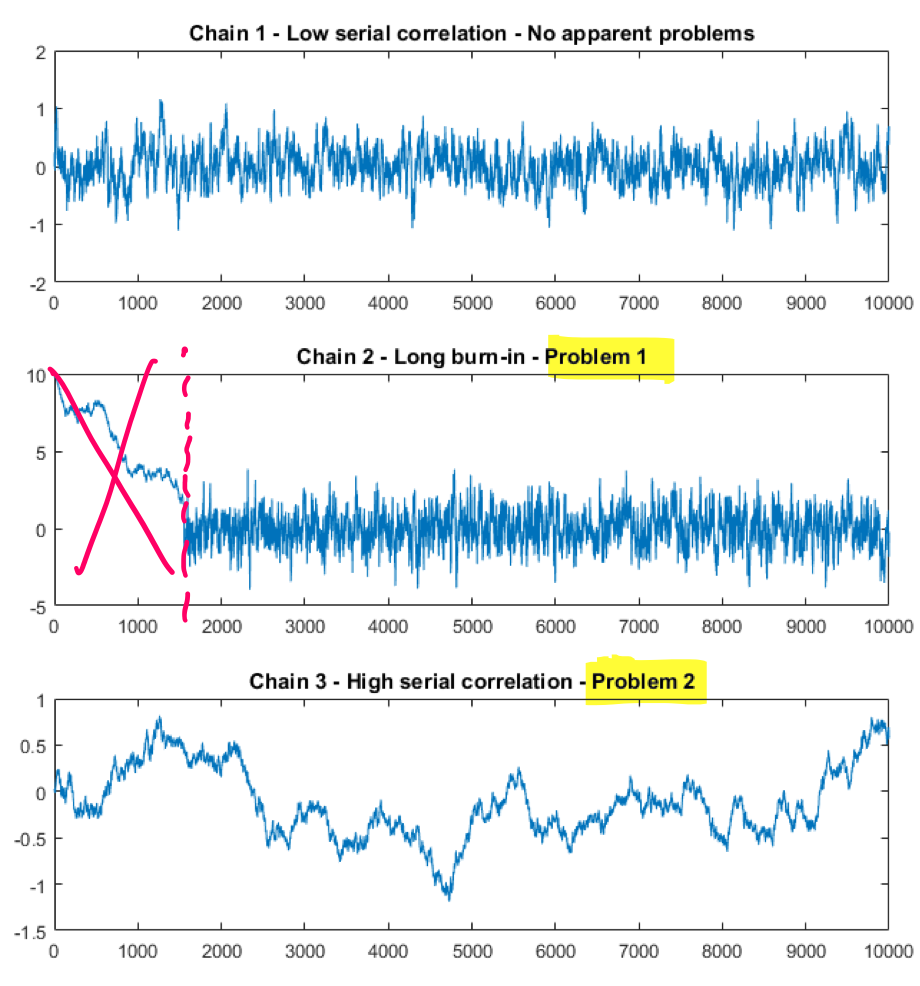
\includegraphics[width=0.5\textwidth]{diag_1.png}
\caption{Diagnostic 1}
\end{figure}
\noindent
The desired output of MCMC should look like the following plots:

\begin{figure}
\centering
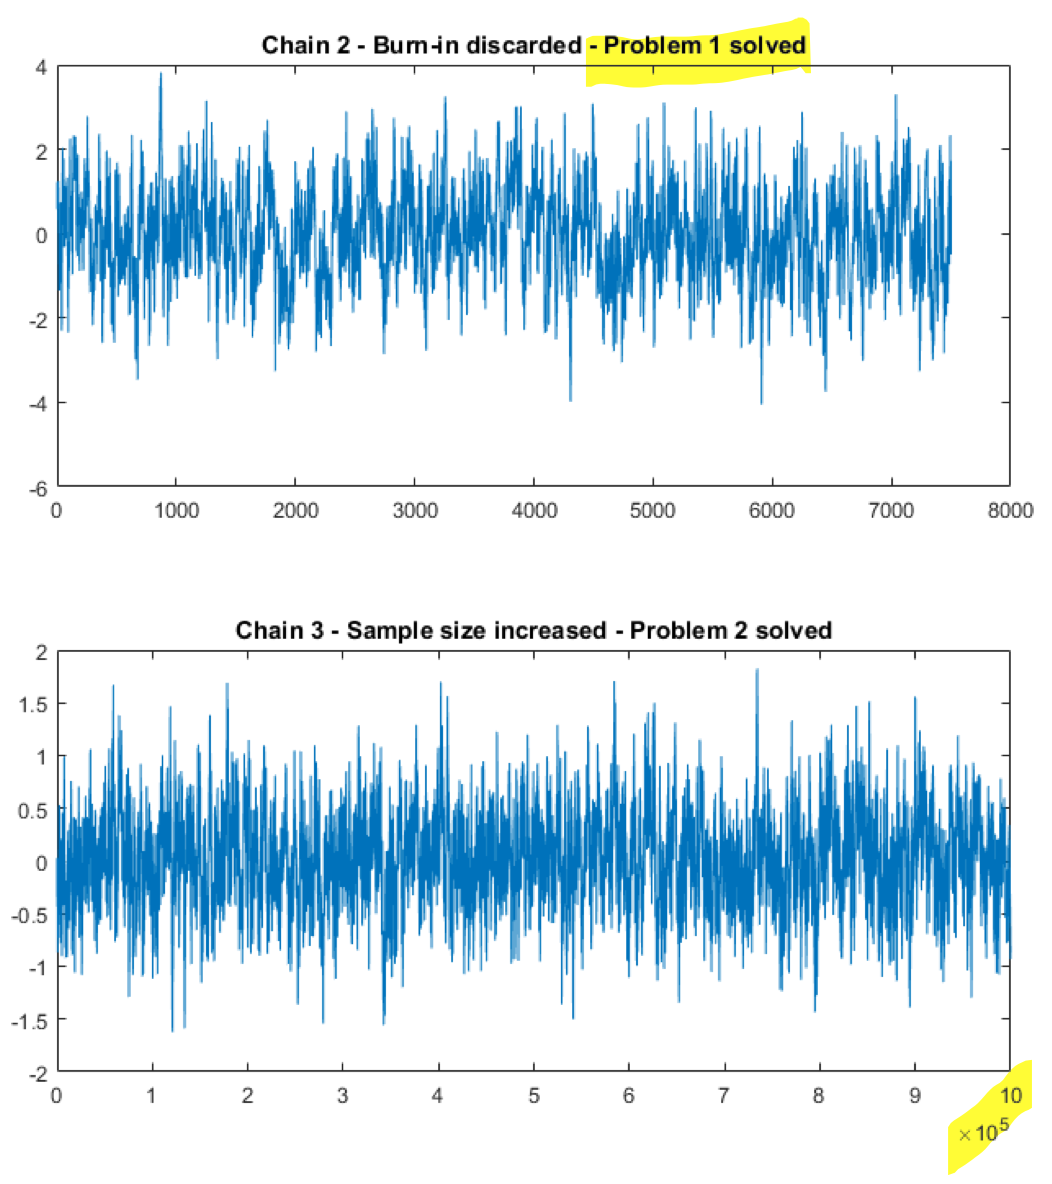
\includegraphics[width=0.5\textwidth]{diag_2.png}
\caption{Diagnostic 2}
\end{figure}

\noindent
Another more analytical approach is \textbf{sample split}. If we split
the plot in different regions, do they have the same mean? Do we observe
consistency? In chain 2 we need longer warm up, in 3 we need more
samples.

\begin{figure}
\centering
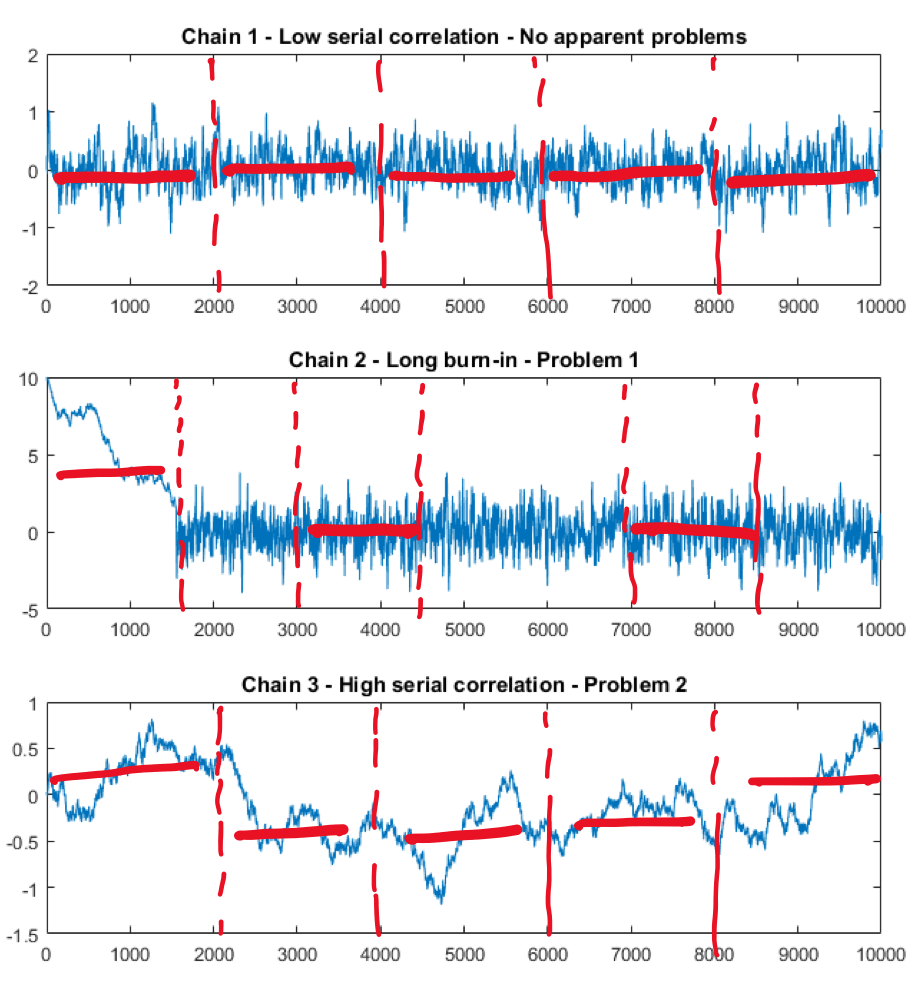
\includegraphics[width=0.5\textwidth]{diag_3.png}
\caption{Diagnostic 3}
\end{figure}
\noindent
Differently from gradient methods, here things are a bit more hard to
interpret. We know that eventually we will reach oscillations around the
global optimum, but we have no guarantee.
\\
\\
\noindent
Diagnostics are based on the observation of the results, so they might
be biased by our belief and they do not provide an easy way to read
``certificate'' of convergence.
\\
\\
\noindent
Another approach may be run more MCMC in parallel and see if they all
converge to the same distribution. However, it is again not a
certificate of convergence to the global optimum.
\\
\\
\noindent
Last observation: constraints and bounds can be included easily in the
proposal distribution or in the likelihood.
